\documentclass[12pt]{article}

\usepackage[utf8]{inputenc}
\usepackage[portuguese]{babel}
\usepackage{indentfirst}
\usepackage[numbers,super]{natbib}
\usepackage{amsmath}
\usepackage{hyperref}
\usepackage{graphicx}

\usepackage{geometry}
\geometry{
	paper = a4paper,
    inner = 3cm,
    outer = 3cm,
    bindingoffset = .5cm,
    top = 2cm,
    bottom = 2cm
}

\begin{document}

% Title page
\begin{titlepage}
\begin{center}

\textbf{\LARGE Universidade Federal de Alagoas } \\[0.5cm]
\textbf{\large Instituto de Computação - IC}\\[0.2cm]

\vspace{20pt}

\vspace{20pt}
\vspace{20pt}
\vspace{20pt}
\vspace{20pt}
\vspace{20pt}
\vspace{20pt}
\vspace{20pt}
\vspace{20pt}

\textbf{\Large Aluno: Danilo Fernandes Costa}\\
\vspace{70pt}
\textbf{\LARGE Relatório de acopanhamento de pesquisa}\\
\vspace{20pt}
\textbf{\Large Análise e processamento de imagens PolSAR}\\
\vspace{70pt}
\textbf{\large Orientador: Alejandro Frery}\\

\vspace{45pt}
\end{center}

\par
\vfill
\begin{center}
\textbf{Maceió - AL}\\
\textbf{2018}
\end{center}

\end{titlepage}

\newpage

%Introducao
\section{Introdução}
Radares de abertura sintética (\textit{Synthetic Aperture Radar} -- SAR) tem a capacidade de capturar imagens da superfície terrestre dia e noite, e quase que independente das condições climáticas~\cite{Shen17}. 
Tal característica se dá devido o imageamento desse tipo de radar ocorrer por meio do envio de ondas eletromagnéticas no espectro de microondas e recepção das mesmas quando refletidas pelo alvo. 
Isso proporciona uma grande vantagem no sensoriamento remoto em relação a radares óticos, o que justifica o seu uso amplo em diversas áreas. 

Além do mais, é possível utilizar a polarização das ondas enviadas e recebidas para caracterizar os objetos monitorados. Tal aperfeiçoamento da tecnologia SAR é chamado SAR Polarimétrico (\textit{Polarimetric SAR} -- PolSAR). 
O dado PolSAR descreve as mudanças do estado de polarização da microonda recebida pelas estruturas e as constantes dielétricas dos objetos~\cite{Ouchi13}, de modo que estas propriedades podem, em princípio, serem extraídas do dado polarimétrico. 

Sistemas SAR geram as imagens da área alvo movendo-se usualmente ao longo de uma trajetoria linear, e transmitindo lateralmente pulsos em direção ao chão, na polarização horizontal (H) ou vertical (V)~\cite{Richards09}. 
A imagem pode ser obtida reunindo todos os dados de intensidade e fase do sinal eletromagnético após ter sido refletido pelo alvo em uma dada polarização~\cite{Pottier09}, onde cada polarização em uma dada cena gera uma imagem complexa.

É comum denotar as imagens complexas das polarizações HH, VV e HV como $S_{\text{HH}}$, $S_{\text{HV}}$ e $S_{\text{VV}}$~\cite{Frery15}, 
% % % ACF Arrume toda a notação confirme a linha acima
onde HV denota um pulso enviado com polarização horizontal e recibido com polarização vertical. Multiplicando o vetor [$S_{HH}$  $S_{HV}$ $S_{VV}$] por seu transposto conjugado [$S_{HH}^*$  $S_{HV}^*$ $S_{VV}^*$]$^t$, obtem-se uma matrix de covariância:
\[
z = 
\begin{bmatrix}
	S_{HH}^*S_{HH} & S_{HH}^*S_{HV} & S_{HH}^*S_{VV}\\
    S_{HV}^*S_{HH} & S_{HV}^*S_{HV} & S_{HV}^*S_{VV}\\
    S_{VV}^*S_{HH} & S_{VV}^*S_{HV} & S_{VV}^*S_{VV}\\
\end{bmatrix},
\]
em que a diagonal principal contem números reais não negativos que representam a intensidade de um sinal medido em uma dada polarização. 
% % % ACF Defina os operadores t e *
%Tomando suas raízes quadradas, obtem-se os valores de amplitude. 
% % % ACF Raramente usaremos amplitude, melhor omitir
Os demais elementos são números complexos e contém informações sobre a diferença de amplitude e fase entre duas polarizações.

Na maioria dos sistemas SAR ou PolSAR, o tamanho da resolução de uma célula é muito maior que o comprimento de onda. 
A medida  do sinal é então uma adição coerente dos ecos de todos os alvos individuais dentro de uma dada célula. 
Dependendo da fase relativa de cada onda retroespelhada, a adição coerente pode ser construtiva ou destrutiva, e isso produz um efeito salpicado sobre as imagens SAR~\cite{Goodman76}. 
A esse efeito dá-se o nome de \textit{speckle}.
% % % Faltou uma transição com o próximo parâgrafo:

O speckle, embora determinístico, é muito difícil de ser tratado dessa forma.
Por se tratar de um fenômeno que depende tipicamente de uma grande quantidade de retroespalhadores por célula de resolução, é mais conveniente tratá-lo como se fosse um processo aleatório.

Portanto, as propriedades do objeto a ser monitorado devem ser extraídas por meio de análises estatísticas dos dados. 
Consequentemente, um modelo estatístico acurado para descrever os dados torna-se de grande relevância para a extração de informações de objetos da superfície terrestre~\cite{Lee99}.

\newpage

\section{Visualização de imagens PolSAR}
As imagens PolSAR podem ser visualizadas por meio da manipulação dos dados que representam a intensidade do sinal de cada uma das polarizações, ou seja, $S_{HH}^*S_{HH}$, $S_{HV}^*S_{HV}$ e $S_{VV}^*S_{VV}$, 
% % % ACF esse é apenas um dos muitos mapeamentos possíveis. Trate isso de forma mais geral, como uma projeção da matriz z em um espaço de cores. Os espaços de cores são tridimensionais, fato que impõe uma redução de dimensionalidade
os quais correspondem respectivamente as bandas RGB. 
O seguinte algoritmo proporciona tal visualização; onde, para fins de otimização, houve compressão da imagem a qual pode ser imaginada como uma segmentação da imagem em matrizes quadradas de ordem cinco e então somente o valor central de cada matriz é selecionado para ser processado e compor a imagem a ser exibida. 

Os dados utilizados estão no formato \texttt{mlc} (calibrated multi-looked) e estão disponíveis no site da \href{https://uavsar.jpl.nasa.gov/cgi-bin/product.pl?jobName=trauns_22551_15087_016_150604_L090_CX_01#data}{UAVSAR}, com sua respectiva documentação. 
Nesta implementação os dados correspondentes a cada uma das bandas foram interpretados como componentes de uma matriz de ordem 5773x3300, 
% % % ACF Use o pacote siunitx 
que é resolução da imagem PolSAR original. 
Esses dados são valores armazenados em ponto flutuante representados por quatro bytes, e para obter uma imagem a partir deles deve-se estabelecer um função de densidade de probabilidade acumulada para cada uma das bandas RGB e aplicá-la para todos os seus valores. 
% % % ACF Não está boa a parte da equalização do histograma. Melhor omitir referências a processamento de imagens
As matrizes resultantes desse processo irão, por fim, compor a imagem PolSAR desejada. 

% % % ACF O algoritmo a seguir faz subamostragem, e você não falou disso

\begin{verbatim}

#Algorithm by John Omena
library("png")

resize <- function(x) {
  return( floor( x / 5 ) )  
}

#Read the file jump 5 columns and rows in the image
read_mlc <- function(file, nrow, ncol) { #Função ainda muito pesada
  
  #Reduce the image to 1/5
  mini_row <- resize( nrow )
  mini_col <- resize( ncol )
  
  matrix <- array(0, dim = c(mini_row, mini_col))
  excess_col <- ncol %% 5
 
  next_byte <- 0
  bytes_per_element <- 4
  col_jump <- 5 #columns to ignore
  row_jump <- 4 #rows to ignore
  
  for(row in 1:mini_row) {
    
    seek(file, where = next_byte, origin = "start")
    
    for(col in 1:mini_col) {
      
      #next line maybe might improved to be more efficient
      matrix[row, col] <- readBin(file, double(), n=1, size = bytes_per_element, endian = "little") # n=1 means to read only one element
      next_byte <- next_byte + bytes_per_element * col_jump 
      
      seek(file, where = next_byte, origin = "start")
      
    }
    
    #Jump the excess of bytes
    next_byte <- next_byte + excess_col * bytes_per_element 
    #Jump 4 rows
    next_byte <- next_byte + row_jump * ncol * bytes_per_element
    
  }
  return(matrix)
   
}
read_mini_RGB_mlc <- function(fileR, fileG, fileB, nrow, ncol) {
  
  dataR <- read_mlc(fileR, nrow, ncol)
  dataG <- read_mlc(fileG, nrow, ncol)
  dataB <- read_mlc(fileB, nrow, ncol)
  
  mini_row <- resize(nrow)
  mini_col <- resize(ncol)
  
  RGB_polsar <- array(0, dim = c(mini_row, mini_col, 3))
  RGB_polsar[,,1] <- dataR
  RGB_polsar[,,2] <- dataG
  RGB_polsar[,,3] <- dataB
  
  return(RGB_polsar)
  
}

#Equalization function to Rdata
Equal_RGB <- function(data, nrow, ncol){
  
  data[,,1] <- matrix(ecdf(data[,,1])(data[,,1]), nrow = nrow,
                      ncol = ncol)
  data[,,2] <- matrix(ecdf(data[,,2])(data[,,2]), nrow = nrow,
                      ncol = ncol)
  data[,,3] <- matrix(ecdf(data[,,3])(data[,,3]), nrow = nrow,
                      ncol = ncol)  
  return(data)
}

nrow <- 5773
ncol <- 3300

fileR <- file("Traunstein_Germany/HHHH.mlc", "rb")
fileG <- file("Traunstein_Germany/HVHV.mlc", "rb")
fileB <- file("Traunstein_Germany/VVVV.mlc", "rb")

UavsarRGB <- read_mini_RGB_mlc(fileR, fileG, fileB, nrow , ncol) #Resolução imagem 5773x3300

#Close files
close(fileR)
close(fileG)
close(fileB)
#Remove file from RAM memory
rm(fileR, fileG, fileB)

mini_row <- resize(nrow)
mini_col <- resize(ncol)

Uavsar_Eq <- Equal_RGB(UavsarRGB, mini_row, mini_col)

writePNG(Uavsar_Eq, target="Traunstein_Germany/image.png")

\end{verbatim}

Resultado do processamento consiste na seguinte imagem de resolução 902x660, a qual teria originalmente uma resolução de 5773x3300:

\begin{figure}[!ht]
	\begin{center}
		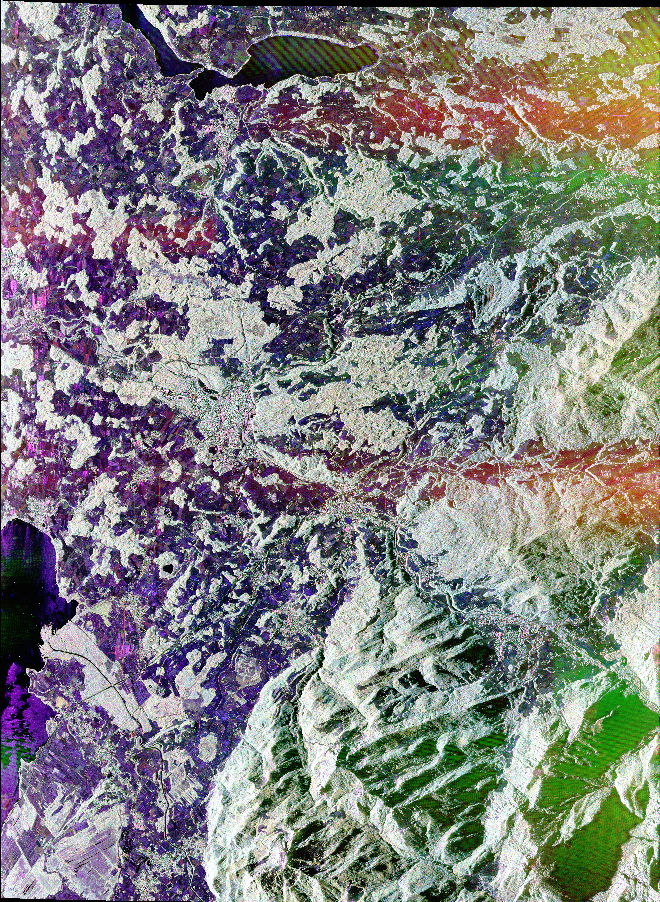
\includegraphics[width = 100mm, scale = 0.5]{../../Images/Report_05_18/traunstein_05_18}
	\end{center}
\end{figure}


\section{Objetivos futuros}

\begin{itemize}

\item Aperfeiçoamento do algoritmo apresentado para visualização de imagens PolSAR de qualquer resolução, bem como melhoria da qualidade da imagem gerada;

\item Desenvolvimento de algoritmo para visualização de segmentos específicos de uma da imagem PolSAR;

\item Estudo de técnicas de processamento de imagens PolSAR;

\item Estudo da modelagem de dados PolSAR por meio da distribuição de probabilidade \textit{$G_{I}^0$}.

\end{itemize}

%Referencias bibliograficas
\bibliographystyle{unsrt}
\bibliography{../../Bibliography/ref}

\end{document}
